textit{RNA-Seq} \cite{Thermes2014, Wang2009, Costa2010, Ozsolak2011} is the most widely used technology to understand gene related regulatory mechanisms in response to stress conditions or drug treatments and progressions of several diseases \cite{Costa2013}.

The main aim of RNA-Seq experiment is to highlight the mainly altered processes (either up-regulated or down-regulated) when comparing two or more conditions at a specific instant in time or in subsequent time points (time-course experiment), and then identify the biological mechanisms regulating such changes.

The general idea underlying the library preparation of an RNA-Seq experiment can be viewed as the conversion of long mRNAs segments in cDNA fragments with RNA or DNA fragmentation. 
To each sequence an adapter for the sequencer is added and a short read is obtained with high-throughput sequencing technology (Figure \ref{fig:rnaseqexp}).


\begin{figure}[h]
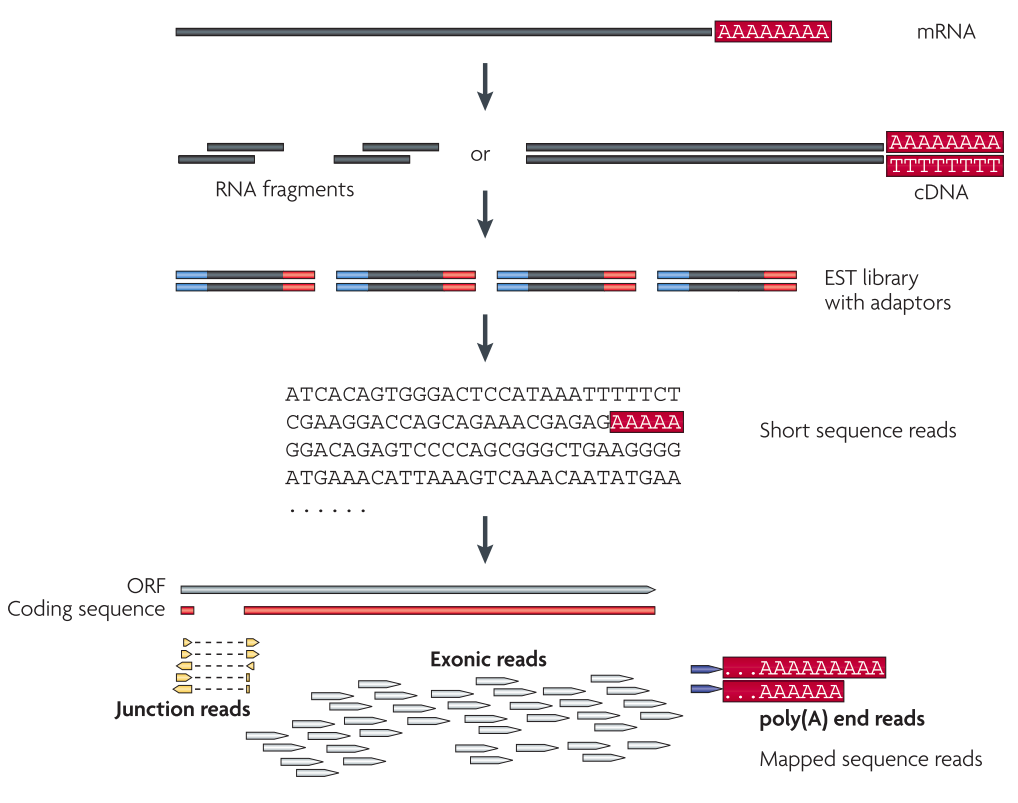
\includegraphics[width=\textwidth,height=\textheight,keepaspectratio]{img/intro/rna-seq.png}
\caption[RNA-Seq experiment]{Representation of an RNA-Seq experiment. \cite{Wang2009}}
\label{fig:rnaseqexp}
\centering
\end{figure}

In order to investigate the experiment, the so-obtained reads have to be analyzed with several tools depending on the particular question the researcher is interested in \cite{Pepke2009, Oshlack2010}.

\begin{figure}[h]
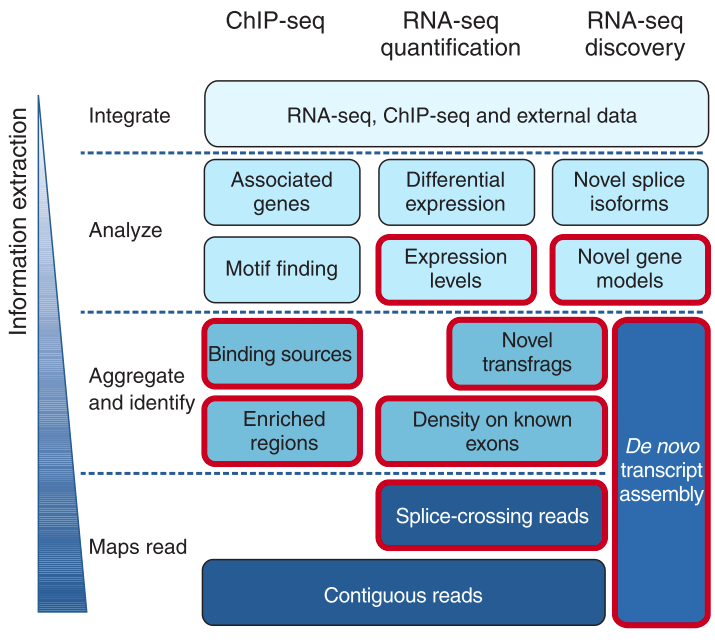
\includegraphics[width=\textwidth,height=\textheight,keepaspectratio]{img/intro/rna-seqan.png}
\caption[RNA-Seq analysis]{Representation of the possible complexity of RNA-Seq analysis. \cite{Pepke2009}}
\label{fig:rnaseqan}
\centering
\end{figure}

In particular we focused on the RNA-seq quantification in case of multiple biological conditions, due to stress, drug treatments, disease specific, etc. where a typical analysis starts from the alignment of the reads on a specie reference genome and the quantification of the mapped reads, producing a count matrix of the samples (on columns) and the genes related features (on the rows), typically identifiers depending on the annotation database used by the analyzer.
Commonly, the counts matrix needs to be filtered from low expressed features and then normalized across the samples, to reduce specific bias for each sample.
Then, it is possible to choose between several methods for the detection of differential expression of the features between the conditions (see section \ref{sec:ticorsermethods}).
Finally, the significant features can be integrated with databases of biological functionalities in order to detect the mostly influenced ones.

